\documentclass[10pt,dvipsnames,enabledeprecatedfontcommands]{scrartcl}
\usepackage{lmodern}
\usepackage{amssymb,amsmath}
\usepackage{ifxetex,ifluatex}
\usepackage{fixltx2e} % provides \textsubscript
\ifnum 0\ifxetex 1\fi\ifluatex 1\fi=0 % if pdftex
  \usepackage[T1]{fontenc}
  \usepackage[utf8]{inputenc}
\else % if luatex or xelatex
  \ifxetex
    \usepackage{mathspec}
  \else
    \usepackage{fontspec}
  \fi
  \defaultfontfeatures{Ligatures=TeX,Scale=MatchLowercase}
\fi
% use upquote if available, for straight quotes in verbatim environments
\IfFileExists{upquote.sty}{\usepackage{upquote}}{}
% use microtype if available
\IfFileExists{microtype.sty}{%
\usepackage[]{microtype}
\UseMicrotypeSet[protrusion]{basicmath} % disable protrusion for tt fonts
}{}
\PassOptionsToPackage{hyphens}{url} % url is loaded by hyperref
\usepackage[unicode=true]{hyperref}
\PassOptionsToPackage{usenames,dvipsnames}{color} % color is loaded by hyperref
\hypersetup{
            pdftitle={Bayesian analysis of the NESTA study of interventions against verbal aggression online},
            pdfauthor={Rafal Urbaniak},
            colorlinks=true,
            linkcolor=Maroon,
            citecolor=Blue,
            urlcolor=blue,
            breaklinks=true}
\urlstyle{same}  % don't use monospace font for urls
\usepackage{color}
\usepackage{fancyvrb}
\newcommand{\VerbBar}{|}
\newcommand{\VERB}{\Verb[commandchars=\\\{\}]}
\DefineVerbatimEnvironment{Highlighting}{Verbatim}{commandchars=\\\{\}}
% Add ',fontsize=\small' for more characters per line
\usepackage{framed}
\definecolor{shadecolor}{RGB}{248,248,248}
\newenvironment{Shaded}{\begin{snugshade}}{\end{snugshade}}
\newcommand{\KeywordTok}[1]{\textcolor[rgb]{0.13,0.29,0.53}{\textbf{#1}}}
\newcommand{\DataTypeTok}[1]{\textcolor[rgb]{0.13,0.29,0.53}{#1}}
\newcommand{\DecValTok}[1]{\textcolor[rgb]{0.00,0.00,0.81}{#1}}
\newcommand{\BaseNTok}[1]{\textcolor[rgb]{0.00,0.00,0.81}{#1}}
\newcommand{\FloatTok}[1]{\textcolor[rgb]{0.00,0.00,0.81}{#1}}
\newcommand{\ConstantTok}[1]{\textcolor[rgb]{0.00,0.00,0.00}{#1}}
\newcommand{\CharTok}[1]{\textcolor[rgb]{0.31,0.60,0.02}{#1}}
\newcommand{\SpecialCharTok}[1]{\textcolor[rgb]{0.00,0.00,0.00}{#1}}
\newcommand{\StringTok}[1]{\textcolor[rgb]{0.31,0.60,0.02}{#1}}
\newcommand{\VerbatimStringTok}[1]{\textcolor[rgb]{0.31,0.60,0.02}{#1}}
\newcommand{\SpecialStringTok}[1]{\textcolor[rgb]{0.31,0.60,0.02}{#1}}
\newcommand{\ImportTok}[1]{#1}
\newcommand{\CommentTok}[1]{\textcolor[rgb]{0.56,0.35,0.01}{\textit{#1}}}
\newcommand{\DocumentationTok}[1]{\textcolor[rgb]{0.56,0.35,0.01}{\textbf{\textit{#1}}}}
\newcommand{\AnnotationTok}[1]{\textcolor[rgb]{0.56,0.35,0.01}{\textbf{\textit{#1}}}}
\newcommand{\CommentVarTok}[1]{\textcolor[rgb]{0.56,0.35,0.01}{\textbf{\textit{#1}}}}
\newcommand{\OtherTok}[1]{\textcolor[rgb]{0.56,0.35,0.01}{#1}}
\newcommand{\FunctionTok}[1]{\textcolor[rgb]{0.00,0.00,0.00}{#1}}
\newcommand{\VariableTok}[1]{\textcolor[rgb]{0.00,0.00,0.00}{#1}}
\newcommand{\ControlFlowTok}[1]{\textcolor[rgb]{0.13,0.29,0.53}{\textbf{#1}}}
\newcommand{\OperatorTok}[1]{\textcolor[rgb]{0.81,0.36,0.00}{\textbf{#1}}}
\newcommand{\BuiltInTok}[1]{#1}
\newcommand{\ExtensionTok}[1]{#1}
\newcommand{\PreprocessorTok}[1]{\textcolor[rgb]{0.56,0.35,0.01}{\textit{#1}}}
\newcommand{\AttributeTok}[1]{\textcolor[rgb]{0.77,0.63,0.00}{#1}}
\newcommand{\RegionMarkerTok}[1]{#1}
\newcommand{\InformationTok}[1]{\textcolor[rgb]{0.56,0.35,0.01}{\textbf{\textit{#1}}}}
\newcommand{\WarningTok}[1]{\textcolor[rgb]{0.56,0.35,0.01}{\textbf{\textit{#1}}}}
\newcommand{\AlertTok}[1]{\textcolor[rgb]{0.94,0.16,0.16}{#1}}
\newcommand{\ErrorTok}[1]{\textcolor[rgb]{0.64,0.00,0.00}{\textbf{#1}}}
\newcommand{\NormalTok}[1]{#1}
\usepackage{graphicx,grffile}
\makeatletter
\def\maxwidth{\ifdim\Gin@nat@width>\linewidth\linewidth\else\Gin@nat@width\fi}
\def\maxheight{\ifdim\Gin@nat@height>\textheight\textheight\else\Gin@nat@height\fi}
\makeatother
% Scale images if necessary, so that they will not overflow the page
% margins by default, and it is still possible to overwrite the defaults
% using explicit options in \includegraphics[width, height, ...]{}
\setkeys{Gin}{width=\maxwidth,height=\maxheight,keepaspectratio}
\IfFileExists{parskip.sty}{%
\usepackage{parskip}
}{% else
\setlength{\parindent}{0pt}
\setlength{\parskip}{6pt plus 2pt minus 1pt}
}
\setlength{\emergencystretch}{3em}  % prevent overfull lines
\providecommand{\tightlist}{%
  \setlength{\itemsep}{0pt}\setlength{\parskip}{0pt}}
\setcounter{secnumdepth}{5}
% Redefines (sub)paragraphs to behave more like sections
\ifx\paragraph\undefined\else
\let\oldparagraph\paragraph
\renewcommand{\paragraph}[1]{\oldparagraph{#1}\mbox{}}
\fi
\ifx\subparagraph\undefined\else
\let\oldsubparagraph\subparagraph
\renewcommand{\subparagraph}[1]{\oldsubparagraph{#1}\mbox{}}
\fi

% set default figure placement to htbp
\makeatletter
\def\fps@figure{htbp}
\makeatother

%\documentclass{article}

% %packages
 \usepackage{booktabs}

\usepackage{multirow}

\usepackage{graphicx}

\usepackage{longtable}
\usepackage{ragged2e}
\usepackage{etex}
%\usepackage{yfonts}
\usepackage{marvosym}
\usepackage[notextcomp]{kpfonts}
\usepackage{nicefrac}
\newcommand*{\QED}{\hfill \footnotesize {\sc Q.e.d.}}
\usepackage{floatrow}

\usepackage[textsize=footnotesize]{todonotes}
%\linespread{1.5}
\usepackage{pdfpages}
\setlength{\parindent}{10pt}
\setlength{\parskip}{1pt}


%language
\usepackage{times}
\usepackage{t1enc}
%\usepackage[utf8x]{inputenc}
%\usepackage[polish]{babel}
%\usepackage{polski}
\usepackage[utf8]{inputenc}
\usepackage{mathptmx}
\usepackage[scaled=0.88]{helvet}


%AMS
\usepackage{amsfonts}
\usepackage{amssymb}
\usepackage{amsthm}
\usepackage{amsmath}
\usepackage{mathtools}

\usepackage{geometry}
 \geometry{a4paper,left=35mm,top=20mm,}


%environments
\newtheorem{fact}{Fact}



%abbreviations
\newcommand{\ra}{\rangle}
\newcommand{\la}{\langle}
\newcommand{\n}{\neg}
\newcommand{\et}{\wedge}
\newcommand{\jt}{\rightarrow}
\newcommand{\ko}[1]{\forall  #1\,}
\newcommand{\ro}{\leftrightarrow}
\newcommand{\exi}[1]{\exists\, {_{#1}}}
\newcommand{\pr}[1]{\mathsf{P}(#1)}
\newcommand{\cost}{\mathsf{cost}}


\newcommand{\odds}{\mathsf{Odds}}
\newcommand{\ind}{\mathsf{Ind}}
\newcommand{\nf}[2]{\nicefrac{#1\,}{#2}}
\newcommand{\R}[1]{\texttt{#1}}
\newcommand{\prr}[1]{\mbox{$\mathtt{P}_{prior}(#1)$}}
\newcommand{\prp}[1]{\mbox{$\mathtt{P}_{posterior}(#1)$}}



\newtheorem{q}{\color{blue}Question}
\newtheorem{lemma}{Lemma}
\newtheorem{theorem}{Theorem}



%technical intermezzo
%---------------------

\newcommand{\intermezzoa}{
	\begin{minipage}[c]{13cm}
	\begin{center}\rule{10cm}{0.4pt}



	\tiny{\sc Optional Content Starts}
	
	\vspace{-1mm}
	
	\rule{10cm}{0.4pt}\end{center}
	\end{minipage}\nopagebreak 
	}


\newcommand{\intermezzob}{\nopagebreak 
	\begin{minipage}[c]{13cm}
	\begin{center}\rule{10cm}{0.4pt}

	\tiny{\sc Optional Content Ends}
	
	\vspace{-1mm}
	
	\rule{10cm}{0.4pt}\end{center}
	\end{minipage}
	}
%--------------------






















\newtheorem*{reply*}{Reply}
\usepackage{enumitem}
\newcommand{\question}[1]{\begin{enumerate}[resume,leftmargin=0cm,labelsep=0cm,align=left]
\item #1
\end{enumerate}}

\usepackage{float}

% \setbeamertemplate{blocks}[rounded][shadow=true]
% \setbeamertemplate{itemize items}[ball]
% \AtBeginPart{}
% \AtBeginSection{}
% \AtBeginSubsection{}
% \AtBeginSubsubsection{}
% \setlength{\emergencystretch}{0em}
% \setlength{\parskip}{0pt}






\usepackage[authoryear]{natbib}

%\bibliographystyle{apalike}
\usepackage{booktabs}
\usepackage{longtable}
\usepackage{array}
\usepackage{multirow}
\usepackage{wrapfig}
\usepackage{float}
\usepackage{colortbl}
\usepackage{pdflscape}
\usepackage{tabu}
\usepackage{threeparttable}
\usepackage{threeparttablex}
\usepackage[normalem]{ulem}
\usepackage{makecell}
\usepackage{xcolor}

\title{Bayesian analysis of the NESTA study of interventions against verbal
aggression online}
\author{Rafal Urbaniak}
\date{}

\begin{document}
\maketitle

\tableofcontents

\section{Exploration}\label{exploration}

Load the dataset and take a look first.

\vspace{1mm} \footnotesize

\begin{Shaded}
\begin{Highlighting}[]
\NormalTok{summaries <-}\StringTok{ }\KeywordTok{read.csv}\NormalTok{(}\DataTypeTok{file =} \StringTok{"datasets/Summaries.csv"}\NormalTok{)}
\KeywordTok{head}\NormalTok{(summaries) }\OperatorTok\StringTok{ }\KeywordTok{kable}\NormalTok{( }\StringTok{"latex"}\NormalTok{, }\DataTypeTok{booktabs =}\NormalTok{ T) }\OperatorTok\StringTok{ }
\StringTok{  }\KeywordTok{kable_styling}\NormalTok{(}\DataTypeTok{latex_options =} \KeywordTok{c}\NormalTok{(}\StringTok{"striped"}\NormalTok{, }\StringTok{"scale_down"}\NormalTok{) ,}\DataTypeTok{font_size =} \DecValTok{9}\NormalTok{)}
\end{Highlighting}
\end{Shaded}

\begin{table}
\centering\begingroup\fontsize{9}{11}\selectfont

\resizebox{\linewidth}{!}{
\begin{tabular}{rlrrrrrrrrrrlr}
\toprule
X & author & AB & AD & AA & CB & CD & CA & Adiff & Cdiff & AdiffS & CdiffS & group & IC\\
\midrule
\cellcolor{gray!6}{1} & \cellcolor{gray!6}{\_swf} & \cellcolor{gray!6}{19} & \cellcolor{gray!6}{1} & \cellcolor{gray!6}{0} & \cellcolor{gray!6}{720} & \cellcolor{gray!6}{25} & \cellcolor{gray!6}{28} & \cellcolor{gray!6}{-19} & \cellcolor{gray!6}{-692} & \cellcolor{gray!6}{-0.0245122} & \cellcolor{gray!6}{-0.3501491} & \cellcolor{gray!6}{normative} & \cellcolor{gray!6}{1}\\
2 & -Allergic & 24 & 24 & 8 & 1614 & 1451 & 1237 & -16 & -377 & 0.0719197 & 0.1057675 & normative & 3\\
\cellcolor{gray!6}{3} & \cellcolor{gray!6}{-funny-username-} & \cellcolor{gray!6}{23} & \cellcolor{gray!6}{6} & \cellcolor{gray!6}{12} & \cellcolor{gray!6}{847} & \cellcolor{gray!6}{497} & \cellcolor{gray!6}{721} & \cellcolor{gray!6}{-11} & \cellcolor{gray!6}{-126} & \cellcolor{gray!6}{0.2326395} & \cellcolor{gray!6}{0.4690535} & \cellcolor{gray!6}{control} & \cellcolor{gray!6}{0}\\
4 & -Johnny- & 18 & 2 & 8 & 1465 & 408 & 684 & -10 & -781 & 0.2647835 & -0.4789637 & empathy & 2\\
\cellcolor{gray!6}{5} & \cellcolor{gray!6}{1secwhileiyeet3} & \cellcolor{gray!6}{15} & \cellcolor{gray!6}{3} & \cellcolor{gray!6}{4} & \cellcolor{gray!6}{1384} & \cellcolor{gray!6}{198} & \cellcolor{gray!6}{120} & \cellcolor{gray!6}{-11} & \cellcolor{gray!6}{-1264} & \cellcolor{gray!6}{0.2326395} & \cellcolor{gray!6}{-1.1780359} & \cellcolor{gray!6}{control} & \cellcolor{gray!6}{0}\\
\addlinespace
6 & 20CharsIsNotEnough & 16 & 10 & 25 & 779 & 907 & 972 & 9 & 193 & 0.8755188 & 0.9307596 & empathy & 4\\
\bottomrule
\end{tabular}}
\endgroup{}
\end{table}

\normalsize

The basic variables we are dealing with are in the following table.

\begin{table}
\centering\begingroup\fontsize{9}{11}\selectfont

\begin{tabular}{ll}
\toprule
variable & explanation\\
\midrule
\cellcolor{gray!6}{AB} & \cellcolor{gray!6}{attacks before (pre-treatment)}\\
AD & attacks during (the treatment period)\\
\cellcolor{gray!6}{AA} & \cellcolor{gray!6}{attacks after (post-treatment)}\\
CB & comments before\\
\cellcolor{gray!6}{CD} & \cellcolor{gray!6}{comments during}\\
\addlinespace
CA & comments after\\
\cellcolor{gray!6}{group} & \cellcolor{gray!6}{treatment group}\\
IC & intervention count\\
\bottomrule
\end{tabular}
\endgroup{}
\end{table}

Further variables are defined in terms of those, in particular, we will
be predicting \textsf{AdiffS} which is the standardized difference
\textsf{AA}-\textsf{AB}, and \textsf{AdiffS}, which is the standardized
difference \textsf{CA}-\textsf{CB}. Before we proceed, we will also
standardize the predictors, and add a numerical index for the group:

\vspace{1mm} \footnotesize

\begin{Shaded}
\begin{Highlighting}[]
\NormalTok{summaries}\OperatorTok{$}\NormalTok{ABS <-}\StringTok{ }\KeywordTok{standardize}\NormalTok{(summaries}\OperatorTok{$}\NormalTok{AB)}
\NormalTok{summaries}\OperatorTok{$}\NormalTok{CBS <-}\StringTok{ }\KeywordTok{standardize}\NormalTok{(summaries}\OperatorTok{$}\NormalTok{CB)}
\NormalTok{summaries}\OperatorTok{$}\NormalTok{AAS <-}\StringTok{ }\KeywordTok{standardize}\NormalTok{(summaries}\OperatorTok{$}\NormalTok{AA)}
\NormalTok{summaries}\OperatorTok{$}\NormalTok{CAS <-}\StringTok{ }\KeywordTok{standardize}\NormalTok{(summaries}\OperatorTok{$}\NormalTok{CA)}
\NormalTok{summaries}\OperatorTok{$}\NormalTok{CDS <-}\StringTok{ }\KeywordTok{standardize}\NormalTok{(summaries}\OperatorTok{$}\NormalTok{CD)}
\NormalTok{summaries}\OperatorTok{$}\NormalTok{ADS <-}\StringTok{ }\KeywordTok{standardize}\NormalTok{(summaries}\OperatorTok{$}\NormalTok{AD)}
\NormalTok{summaries}\OperatorTok{$}\NormalTok{group <-}\StringTok{ }\KeywordTok{as.factor}\NormalTok{(summaries}\OperatorTok{$}\NormalTok{group)}
\NormalTok{summaries}\OperatorTok{$}\NormalTok{groupID <-}\StringTok{  }\KeywordTok{as.integer}\NormalTok{( }\KeywordTok{as.factor}\NormalTok{(summaries}\OperatorTok{$}\NormalTok{group) )}
\end{Highlighting}
\end{Shaded}

\normalsize

First, let's take a look at the distribution of \textsf{IC} in the
treatment groups:

\vspace{1mm} \footnotesize

\begin{Shaded}
\begin{Highlighting}[]
\KeywordTok{ggplot}\NormalTok{(summaries[summaries}\OperatorTok{$}\NormalTok{group }\OperatorTok{!=}\StringTok{ "control"}\NormalTok{,], }\KeywordTok{aes}\NormalTok{(}\DataTypeTok{x =}\NormalTok{ IC, }\DataTypeTok{fill =}\NormalTok{ group))}\OperatorTok{+}
\StringTok{  }\KeywordTok{geom_bar}\NormalTok{()}\OperatorTok{+}\KeywordTok{theme_tufte}\NormalTok{()}\OperatorTok{+}
\StringTok{  }\KeywordTok{xlab}\NormalTok{(}\StringTok{"interventions received"}\NormalTok{)}\OperatorTok{+}
\StringTok{  }\KeywordTok{labs}\NormalTok{(}\DataTypeTok{title =} \StringTok{"Intervention counts in treatment groups"}\NormalTok{)}\OperatorTok{+}
\StringTok{  }\KeywordTok{scale_x_continuous}\NormalTok{(}\DataTypeTok{breaks =} \KeywordTok{seq}\NormalTok{(}\DecValTok{0}\NormalTok{,}\DecValTok{40}\NormalTok{,}\DecValTok{5}\NormalTok{))}
\end{Highlighting}
\end{Shaded}

\begin{center}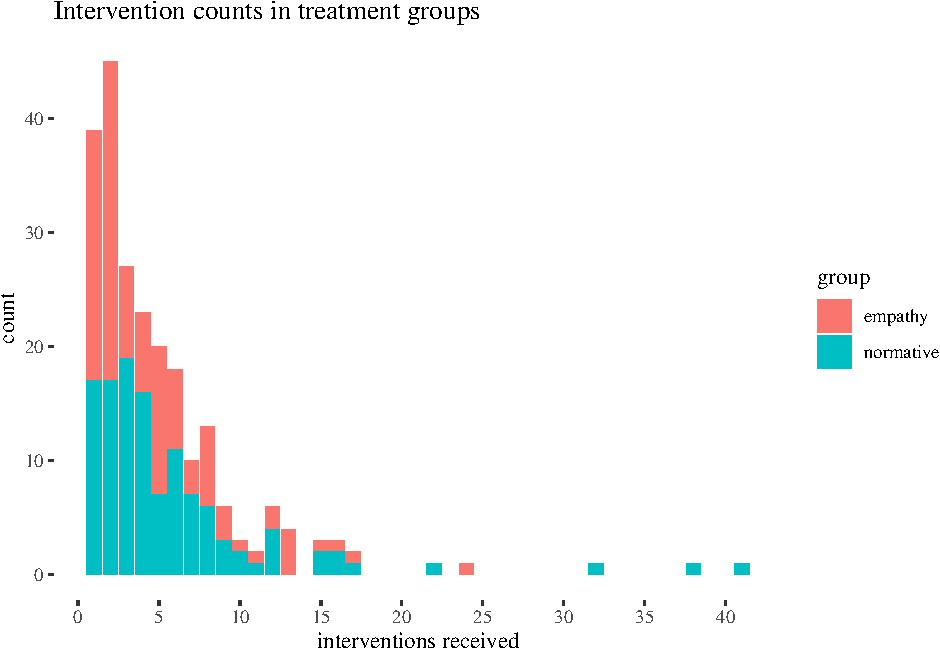
\includegraphics[width=1\linewidth]{bayesianReport_files/figure-latex/treatmentHist-1} \end{center}

\normalsize

\todo{Note there were much more empathetic interventions, this needs an explanation}

\todo{Question: intervention counts by group}

Second, when we look at the distribution of standardized difference in
attacks, when restricted to (-1,1), the peaks of distributions are
shifted a bit, with lowest median for the normative group, but not too
much:

\vspace{1mm} \footnotesize

\begin{Shaded}
\begin{Highlighting}[]
\NormalTok{violAdiffS <-}\StringTok{ }\KeywordTok{ggplot}\NormalTok{(summaries, }\KeywordTok{aes}\NormalTok{(}\DataTypeTok{x=}\NormalTok{group, }\DataTypeTok{y =}\NormalTok{ AdiffS))}\OperatorTok{+}
\StringTok{  }\KeywordTok{geom_violin}\NormalTok{() }\OperatorTok{+}\KeywordTok{theme_tufte}\NormalTok{() }
\NormalTok{violJoint <-}\StringTok{ }\KeywordTok{ggarrange}\NormalTok{(violAdiffS}\OperatorTok{+}\KeywordTok{ggtitle}\NormalTok{(}\StringTok{"whole range"}\NormalTok{),}
\NormalTok{              violAdiffS }\OperatorTok{+}\StringTok{ }\KeywordTok{ylim}\NormalTok{(}\KeywordTok{c}\NormalTok{(}\OperatorTok{-}\DecValTok{1}\NormalTok{,}\DecValTok{1}\NormalTok{))}\OperatorTok{+}\KeywordTok{geom_boxplot}\NormalTok{(}\DataTypeTok{width =} \FloatTok{.2}\NormalTok{)}\OperatorTok{+}
\StringTok{              }\KeywordTok{ggtitle}\NormalTok{(}\StringTok{"restricted to (-1,1)"}\NormalTok{)) }
\end{Highlighting}
\end{Shaded}

\begin{verbatim}
## Warning: Removed 58 rows containing non-finite values (stat_ydensity).
\end{verbatim}

\begin{verbatim}
## Warning: Removed 58 rows containing non-finite values (stat_boxplot).
\end{verbatim}

\begin{Shaded}
\begin{Highlighting}[]
\NormalTok{violJointTitled <-}\StringTok{ }\KeywordTok{annotate_figure}\NormalTok{(violJoint, }
  \DataTypeTok{top =} \KeywordTok{text_grob}\NormalTok{(}\StringTok{"Empirical distribution of change in attacks (standardized)"}\NormalTok{,}
                  \DataTypeTok{size =} \DecValTok{12}\NormalTok{))}
\NormalTok{violJointTitled}
\end{Highlighting}
\end{Shaded}

\begin{center}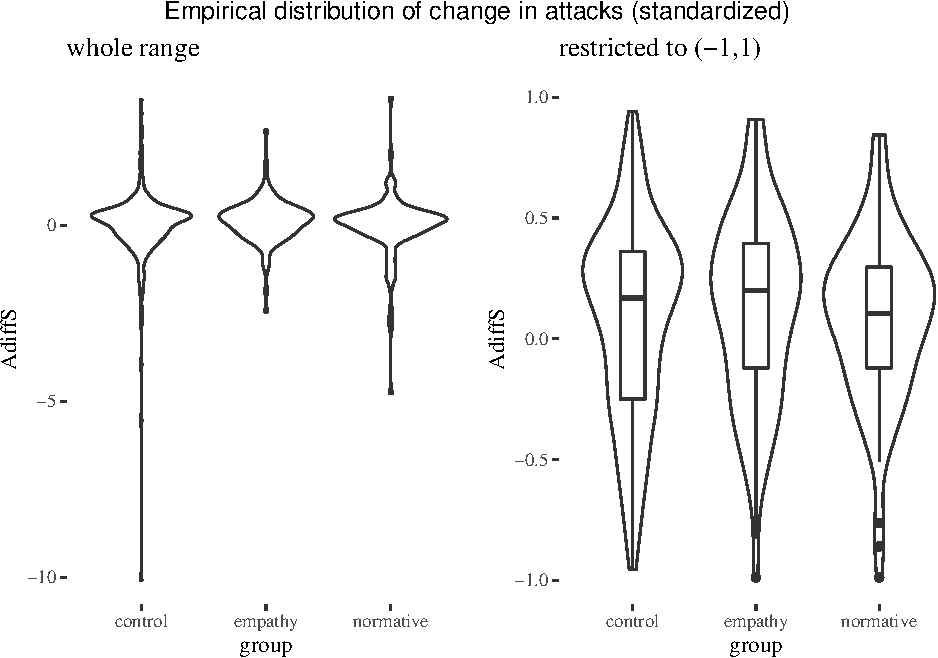
\includegraphics[width=1\linewidth]{bayesianReport_files/figure-latex/violEmpiricalAdiff-1} \end{center}

\normalsize

Analogous plot for comments does not reveal this slight downward shift
for normative, but otherwise the visualisation migth suggest no strong
impact of interventions on attacks, and no impact on comments.

\vspace{1mm} \footnotesize

\begin{Shaded}
\begin{Highlighting}[]
\NormalTok{violCdiffS <-}\StringTok{ }\KeywordTok{ggplot}\NormalTok{(summaries, }\KeywordTok{aes}\NormalTok{(}\DataTypeTok{x=}\NormalTok{group, }\DataTypeTok{y =}\NormalTok{ CdiffS))}\OperatorTok{+}
\StringTok{  }\KeywordTok{geom_violin}\NormalTok{() }\OperatorTok{+}\KeywordTok{theme_tufte}\NormalTok{() }
\NormalTok{violJointC <-}\StringTok{ }\KeywordTok{ggarrange}\NormalTok{(violCdiffS}\OperatorTok{+}\KeywordTok{ggtitle}\NormalTok{(}\StringTok{"whole range"}\NormalTok{),}
\NormalTok{              violCdiffS }\OperatorTok{+}\StringTok{ }\KeywordTok{ylim}\NormalTok{(}\KeywordTok{c}\NormalTok{(}\OperatorTok{-}\DecValTok{1}\NormalTok{,}\DecValTok{1}\NormalTok{))}\OperatorTok{+}\KeywordTok{geom_boxplot}\NormalTok{(}\DataTypeTok{width =} \FloatTok{.2}\NormalTok{)}\OperatorTok{+}
\StringTok{              }\KeywordTok{ggtitle}\NormalTok{(}\StringTok{"restricted to (-1,1)"}\NormalTok{)) }
\end{Highlighting}
\end{Shaded}

\begin{verbatim}
## Warning: Removed 90 rows containing non-finite values (stat_ydensity).
\end{verbatim}

\begin{verbatim}
## Warning: Removed 90 rows containing non-finite values (stat_boxplot).
\end{verbatim}

\begin{Shaded}
\begin{Highlighting}[]
\NormalTok{violJointCTitled <-}\StringTok{ }\KeywordTok{annotate_figure}\NormalTok{(violJoint, }
  \DataTypeTok{top =} \KeywordTok{text_grob}\NormalTok{(}\StringTok{"Empirical distribution of change in comments (standardized)"}\NormalTok{,}
                  \DataTypeTok{size =} \DecValTok{12}\NormalTok{))}
\NormalTok{violJointCTitled}
\end{Highlighting}
\end{Shaded}

\begin{center}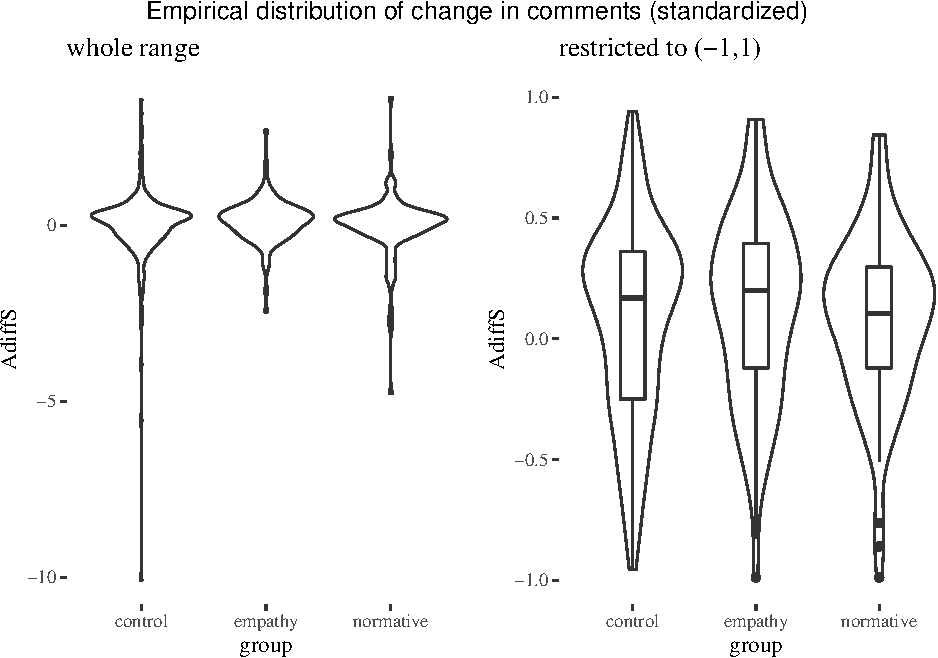
\includegraphics[width=1\linewidth]{bayesianReport_files/figure-latex/violEpmiricalCdiff-1} \end{center}

\normalsize

However, plotting changes against intervention counts reveals that
restricting attention to various activity levels drastically changes the
regression lines.

\vspace{1mm} \footnotesize

\begin{Shaded}
\begin{Highlighting}[]
\NormalTok{icplot1 <-}\StringTok{ }\KeywordTok{ggplot}\NormalTok{(summaries, }\KeywordTok{aes}\NormalTok{(}\DataTypeTok{x =}\NormalTok{ IC, }\DataTypeTok{y =}\NormalTok{ AdiffS, }\DataTypeTok{color =}\NormalTok{ group, }\DataTypeTok{fill =}\NormalTok{ group))}\OperatorTok{+}
\StringTok{  }\KeywordTok{geom_jitter}\NormalTok{(}\DataTypeTok{alpha =} \FloatTok{0.6}\NormalTok{, }\DataTypeTok{size =}\NormalTok{.}\DecValTok{8}\NormalTok{)}\OperatorTok{+}\KeywordTok{theme_tufte}\NormalTok{()}\OperatorTok{+}
\StringTok{  }\KeywordTok{geom_smooth}\NormalTok{(}\DataTypeTok{alpha =} \FloatTok{0.2}\NormalTok{, }\DataTypeTok{method =} \StringTok{"lm"}\NormalTok{)}\OperatorTok{+}
\StringTok{  }\KeywordTok{xlim}\NormalTok{(}\KeywordTok{c}\NormalTok{(}\DecValTok{0}\NormalTok{,}\DecValTok{25}\NormalTok{))}\OperatorTok{+}\KeywordTok{ylim}\NormalTok{(}\KeywordTok{c}\NormalTok{(}\OperatorTok{-}\DecValTok{2}\NormalTok{,}\DecValTok{2}\NormalTok{))}\OperatorTok{+}
\StringTok{  }\KeywordTok{ggtitle}\NormalTok{(}\StringTok{"sd restricted to (-2,2)"}\NormalTok{)}\OperatorTok{+}
\StringTok{  }\KeywordTok{theme}\NormalTok{(}\DataTypeTok{legend.position =} \KeywordTok{c}\NormalTok{(}\FloatTok{0.65}\NormalTok{, }\FloatTok{0.1}\NormalTok{))}

\NormalTok{icplot2 <-}\StringTok{  }\KeywordTok{ggplot}\NormalTok{(summaries, }\KeywordTok{aes}\NormalTok{(}\DataTypeTok{x =}\NormalTok{ IC, }\DataTypeTok{y =}\NormalTok{ AdiffS, }\DataTypeTok{color =}\NormalTok{ group, }\DataTypeTok{fill =}\NormalTok{ group))}\OperatorTok{+}
\StringTok{  }\KeywordTok{geom_jitter}\NormalTok{(}\DataTypeTok{alpha =} \FloatTok{0.6}\NormalTok{, }\DataTypeTok{size =}\NormalTok{.}\DecValTok{8}\NormalTok{)}\OperatorTok{+}\KeywordTok{theme_tufte}\NormalTok{()}\OperatorTok{+}
\StringTok{  }\KeywordTok{geom_smooth}\NormalTok{(}\DataTypeTok{alpha =} \FloatTok{0.2}\NormalTok{, }\DataTypeTok{method =} \StringTok{"lm"}\NormalTok{)}\OperatorTok{+}
\StringTok{  }\KeywordTok{xlim}\NormalTok{(}\KeywordTok{c}\NormalTok{(}\DecValTok{0}\NormalTok{,}\DecValTok{25}\NormalTok{))}\OperatorTok{+}\KeywordTok{ylim}\NormalTok{(}\KeywordTok{c}\NormalTok{(}\OperatorTok{-}\DecValTok{1}\NormalTok{,}\DecValTok{1}\NormalTok{))}\OperatorTok{+}\KeywordTok{ggtitle}\NormalTok{(}\StringTok{"sd restricted to (-1,1)"}\NormalTok{)}\OperatorTok{+}
\StringTok{  }\KeywordTok{theme}\NormalTok{(}\DataTypeTok{legend.position =} \KeywordTok{c}\NormalTok{(}\FloatTok{0.65}\NormalTok{, }\FloatTok{0.1}\NormalTok{))}

\NormalTok{icplotJoint <-}\StringTok{ }\KeywordTok{ggarrange}\NormalTok{(icplot1, icplot2) }
\NormalTok{icplotTitled <-}\StringTok{ }\KeywordTok{annotate_figure}\NormalTok{(icplotJoint, }
  \DataTypeTok{top =} \KeywordTok{text_grob}\NormalTok{(}\StringTok{"Change in attacks (standardized) vs interventions received"}\NormalTok{,  }\DataTypeTok{size =} \DecValTok{12}\NormalTok{))}
\NormalTok{icplotTitled}
\end{Highlighting}
\end{Shaded}

\begin{center}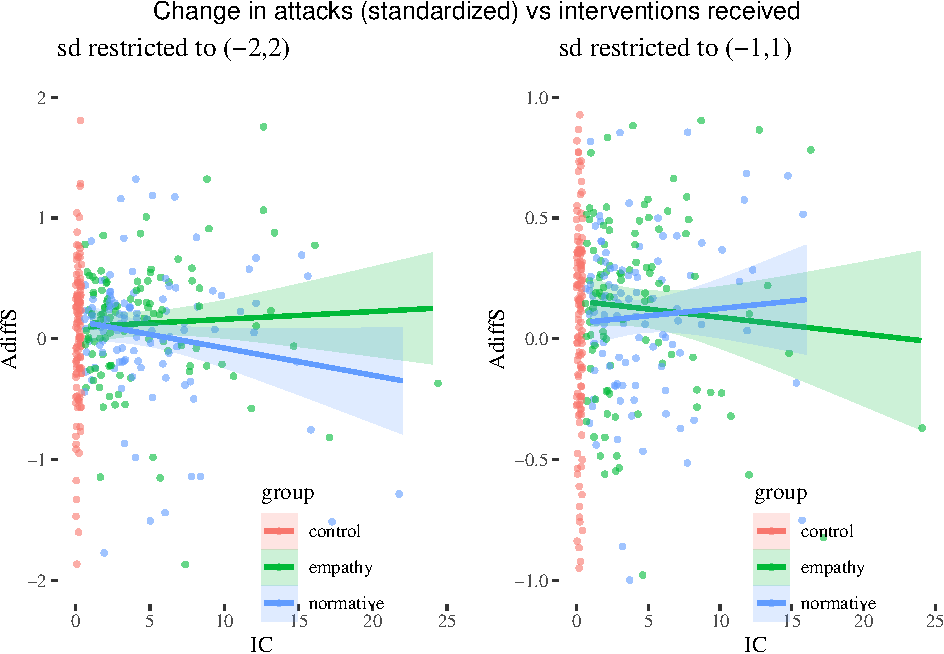
\includegraphics[width=1\linewidth]{bayesianReport_files/figure-latex/ic-1} \end{center}

\normalsize

Some interactions are also suggested by the differences in linear
smoothing when attention is restricted when it comes to change in
comments.

\vspace{1mm} \footnotesize

\begin{Shaded}
\begin{Highlighting}[]
\NormalTok{icCplot1 <-}\StringTok{ }\KeywordTok{ggplot}\NormalTok{(summaries, }\KeywordTok{aes}\NormalTok{(}\DataTypeTok{x =}\NormalTok{ IC, }\DataTypeTok{y =}\NormalTok{ CdiffS, }\DataTypeTok{color =}\NormalTok{ group, }\DataTypeTok{fill =}\NormalTok{ group))}\OperatorTok{+}
\StringTok{  }\KeywordTok{geom_jitter}\NormalTok{(}\DataTypeTok{alpha =} \FloatTok{0.6}\NormalTok{, }\DataTypeTok{size =}\NormalTok{.}\DecValTok{8}\NormalTok{)}\OperatorTok{+}\KeywordTok{theme_tufte}\NormalTok{()}\OperatorTok{+}
\StringTok{  }\KeywordTok{geom_smooth}\NormalTok{(}\DataTypeTok{alpha =} \FloatTok{0.2}\NormalTok{, }\DataTypeTok{method =} \StringTok{"lm"}\NormalTok{)}\OperatorTok{+}
\StringTok{  }\KeywordTok{xlim}\NormalTok{(}\KeywordTok{c}\NormalTok{(}\DecValTok{0}\NormalTok{,}\DecValTok{25}\NormalTok{))}\OperatorTok{+}\KeywordTok{ylim}\NormalTok{(}\KeywordTok{c}\NormalTok{(}\OperatorTok{-}\DecValTok{2}\NormalTok{,}\DecValTok{2}\NormalTok{))}\OperatorTok{+}
\StringTok{  }\KeywordTok{ggtitle}\NormalTok{(}\StringTok{"sd restricted to (-2,2)"}\NormalTok{)}\OperatorTok{+}
\StringTok{  }\KeywordTok{theme}\NormalTok{(}\DataTypeTok{legend.position =} \KeywordTok{c}\NormalTok{(}\FloatTok{0.65}\NormalTok{, }\FloatTok{0.1}\NormalTok{))}

\NormalTok{icCplot2 <-}\StringTok{  }\KeywordTok{ggplot}\NormalTok{(summaries, }\KeywordTok{aes}\NormalTok{(}\DataTypeTok{x =}\NormalTok{ IC, }\DataTypeTok{y =}\NormalTok{ CdiffS, }\DataTypeTok{color =}\NormalTok{ group, }\DataTypeTok{fill =}\NormalTok{ group))}\OperatorTok{+}
\StringTok{  }\KeywordTok{geom_jitter}\NormalTok{(}\DataTypeTok{alpha =} \FloatTok{0.6}\NormalTok{, }\DataTypeTok{size =}\NormalTok{.}\DecValTok{8}\NormalTok{)}\OperatorTok{+}\KeywordTok{theme_tufte}\NormalTok{()}\OperatorTok{+}
\StringTok{  }\KeywordTok{geom_smooth}\NormalTok{(}\DataTypeTok{alpha =} \FloatTok{0.2}\NormalTok{, }\DataTypeTok{method =} \StringTok{"lm"}\NormalTok{)}\OperatorTok{+}
\StringTok{  }\KeywordTok{xlim}\NormalTok{(}\KeywordTok{c}\NormalTok{(}\DecValTok{0}\NormalTok{,}\DecValTok{25}\NormalTok{))}\OperatorTok{+}\KeywordTok{ylim}\NormalTok{(}\KeywordTok{c}\NormalTok{(}\OperatorTok{-}\DecValTok{1}\NormalTok{,}\DecValTok{1}\NormalTok{))}\OperatorTok{+}\KeywordTok{ggtitle}\NormalTok{(}\StringTok{"sd restricted to (-1,1)"}\NormalTok{)}\OperatorTok{+}
\StringTok{  }\KeywordTok{theme}\NormalTok{(}\DataTypeTok{legend.position =} \KeywordTok{c}\NormalTok{(}\FloatTok{0.65}\NormalTok{, }\FloatTok{0.1}\NormalTok{))}

\NormalTok{icCplotJoint <-}\StringTok{ }\KeywordTok{ggarrange}\NormalTok{(icCplot1, icCplot2) }
\NormalTok{icCplotTitled <-}\StringTok{ }\KeywordTok{annotate_figure}\NormalTok{(icCplotJoint, }
  \DataTypeTok{top =} \KeywordTok{text_grob}\NormalTok{(}\StringTok{"Change in comments (standardized) vs interventions received"}\NormalTok{,}
   \DataTypeTok{size =} \DecValTok{12}\NormalTok{))}
\NormalTok{icCplotTitled}
\end{Highlighting}
\end{Shaded}

\begin{center}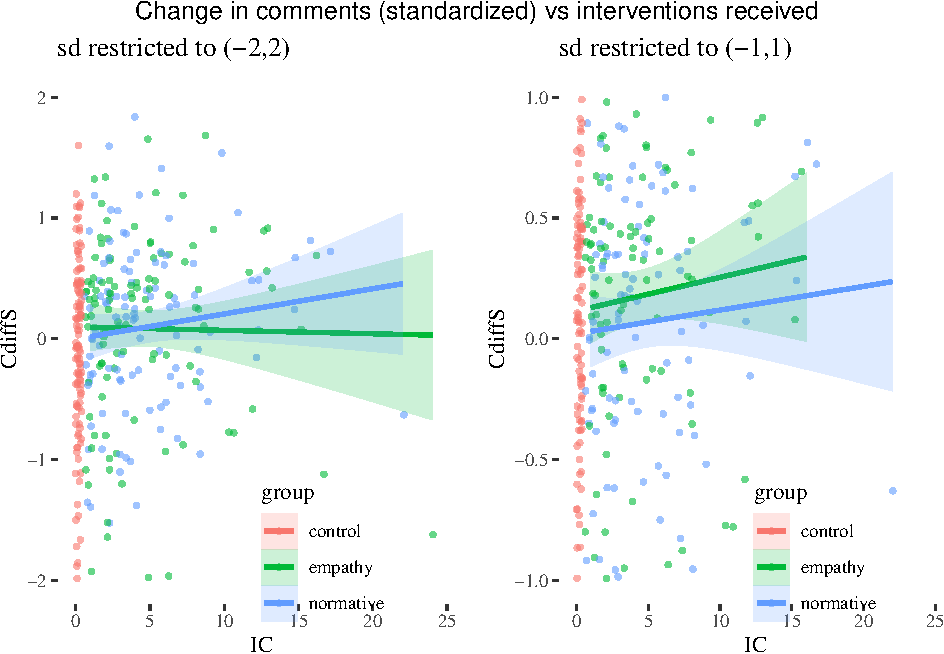
\includegraphics[width=1\linewidth]{bayesianReport_files/figure-latex/icc-1} \end{center}

\normalsize

This suggests we should keep an eye out for interactions in the
analysis, and that the intial comparison of means or medians between
groups might be misleading if the effects in different volume groups are
different and cancel each other.

Now, let's inspect correlations between the variables involved in the
model:

\vspace{1mm} \footnotesize

\begin{Shaded}
\begin{Highlighting}[]
\NormalTok{summariesCorr <-}\StringTok{ }\KeywordTok{select}\NormalTok{(summaries, IC, ABS, CBS, AAS, CAS, CDS, ADS)}
\KeywordTok{ggcorr}\NormalTok{(summariesCorr, }\DataTypeTok{method =} \KeywordTok{c}\NormalTok{(}\StringTok{"pairwise"}\NormalTok{),}
       \DataTypeTok{digits =} \DecValTok{4}\NormalTok{, }\DataTypeTok{low =} \StringTok{"steelblue"}\NormalTok{, }\DataTypeTok{mid =} \StringTok{"white"}\NormalTok{,}
       \DataTypeTok{high =} \StringTok{"darkred"}\NormalTok{, }\DataTypeTok{midpoint =}\DecValTok{0}\NormalTok{,}
       \DataTypeTok{geom =} \StringTok{"tile"}\NormalTok{, }\DataTypeTok{label =} \OtherTok{TRUE}\NormalTok{, }\DataTypeTok{label_size=}\DecValTok{4}\NormalTok{, }\DataTypeTok{label_round =}\DecValTok{2}\NormalTok{, }\DataTypeTok{layout.exp =}\DecValTok{1}\NormalTok{,}
       \DataTypeTok{label_alpha =} \OtherTok{FALSE}\NormalTok{,}\DataTypeTok{hjust =} \FloatTok{0.75}\NormalTok{)}
\end{Highlighting}
\end{Shaded}

\begin{center}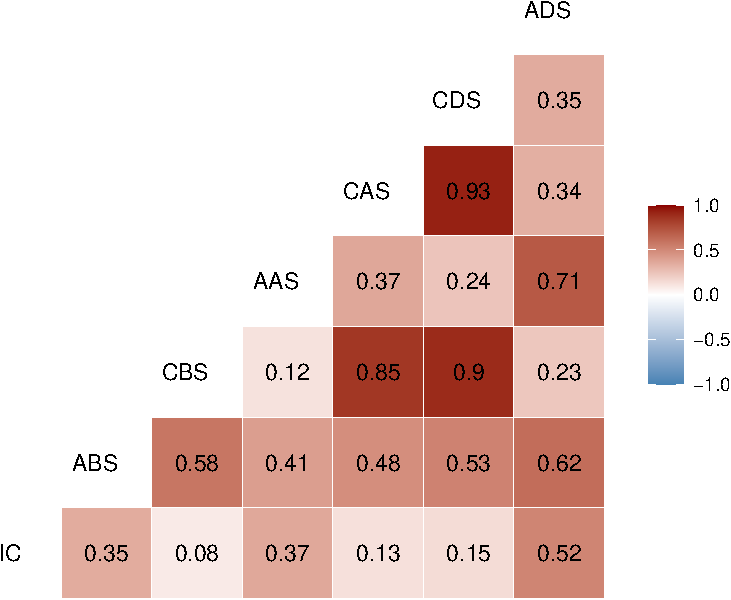
\includegraphics[width=1\linewidth]{bayesianReport_files/figure-latex/correlations-1} \end{center}

\normalsize

This tells us that almost no predictors are strongly correlated, except
for pairs \textsf{CBS}-\textsf{CDS}, so we drop CDS from the analysis
and avoid using them in the same model to avoid multicolinearity issues.
These are just comments during the intervention period, which,
unsurprisingly are also a good proxy for comments before and comments
after.

\section{Causal inference}\label{causal-inference}

To identify the right variables to condition (or not condition) on to
identify the causal effect of the interventions, we first need to think
about the causal structure of the problem. Here's a plausible causal
structure that we will be working with:

\vspace{1mm} \footnotesize

\begin{Shaded}
\begin{Highlighting}[]
\NormalTok{dag <-}\StringTok{ }\KeywordTok{dagitty}\NormalTok{(}\StringTok{"}
\StringTok{  dag\{}
\StringTok{  CDS -> ADS -> IC  ons}
\StringTok{               U [unobserved]   }
\StringTok{               U -> CBS -> ABS  }
\StringTok{               U -> ABS        }
\StringTok{               U -> CDS -> ADS  }
\StringTok{               U -> ADS         }
\StringTok{               U -> CAS -> AAS    }
\StringTok{               U -> AAS                        }
\StringTok{               IC -> AAS        }
\StringTok{               IC -> CAS        }
\StringTok{               IT -> CAS        }
\StringTok{               IT -> AAS}
\StringTok{               CBS -> CDS -> CAS}
\StringTok{               ABS -> ADS -> AAS}
\StringTok{               \}"}\NormalTok{)}
\KeywordTok{set.seed}\NormalTok{(}\DecValTok{123}\NormalTok{)}
\KeywordTok{drawdag}\NormalTok{(dag)}
\end{Highlighting}
\end{Shaded}

\begin{center}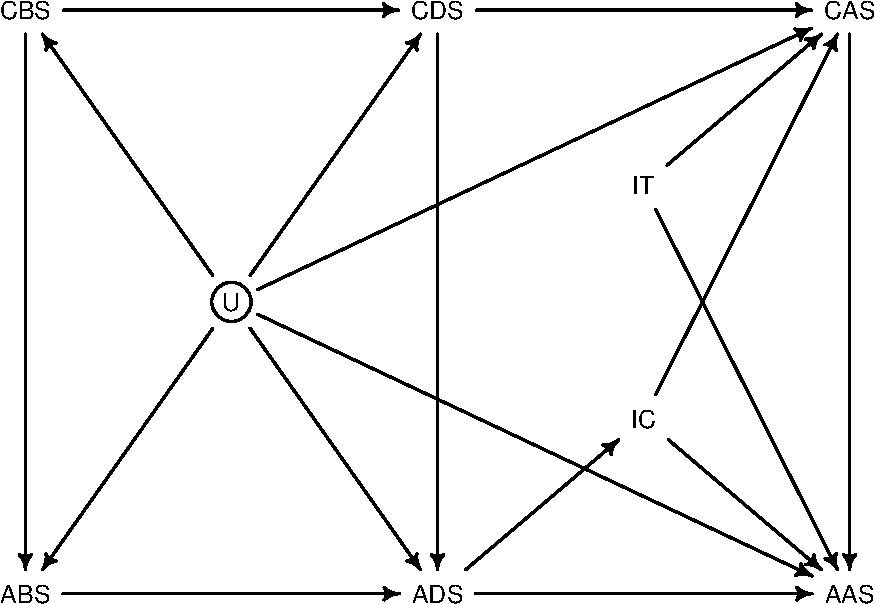
\includegraphics[width=1\linewidth]{bayesianReport_files/figure-latex/dag1-1} \end{center}

\normalsize

Comments during impact attacks during, which trigger interventions.
Unmeasured user features cause comments before, which impact attacks
before, and also attacks before directly. Comments during (their impact
on ADS is areadly included) impact attacks during during directly and
comments after, which impact attacks after and attacks after directly.
Intervention count impacts attacks after and comments after. The same
directions of impact are included for intervention type. Finally,
comments through time are connected causally, and so are attacks.

We already know not to condition on CDS if we condition on CAS or CBS.
What else? \textsf{IT} has no bacwkard paths, but \textsf{IC} does.
Let's identify all paths from \textsf{IC} to \textsf{AAS}:

\vspace{1mm} \footnotesize

\begin{Shaded}
\begin{Highlighting}[]
\KeywordTok{paths}\NormalTok{(dag, }\DataTypeTok{from =} \KeywordTok{c}\NormalTok{(}\StringTok{"IC"}\NormalTok{), }\DataTypeTok{to =} \StringTok{"AAS"}\NormalTok{)}
\end{Highlighting}
\end{Shaded}

\begin{verbatim}
## $paths
##  [1] "IC -> AAS"                                              
##  [2] "IC -> CAS -> AAS"                                       
##  [3] "IC -> CAS <- CDS -> ADS -> AAS"                         
##  [4] "IC -> CAS <- CDS -> ADS <- ABS <- CBS <- U -> AAS"      
##  [5] "IC -> CAS <- CDS -> ADS <- ABS <- U -> AAS"             
##  [6] "IC -> CAS <- CDS -> ADS <- U -> AAS"                    
##  [7] "IC -> CAS <- CDS <- CBS -> ABS -> ADS -> AAS"           
##  [8] "IC -> CAS <- CDS <- CBS -> ABS -> ADS <- U -> AAS"      
##  [9] "IC -> CAS <- CDS <- CBS -> ABS <- U -> AAS"             
## [10] "IC -> CAS <- CDS <- CBS -> ABS <- U -> ADS -> AAS"      
## [11] "IC -> CAS <- CDS <- CBS <- U -> AAS"                    
## [12] "IC -> CAS <- CDS <- CBS <- U -> ABS -> ADS -> AAS"      
## [13] "IC -> CAS <- CDS <- CBS <- U -> ADS -> AAS"             
## [14] "IC -> CAS <- CDS <- U -> AAS"                           
## [15] "IC -> CAS <- CDS <- U -> ABS -> ADS -> AAS"             
## [16] "IC -> CAS <- CDS <- U -> ADS -> AAS"                    
## [17] "IC -> CAS <- CDS <- U -> CBS -> ABS -> ADS -> AAS"      
## [18] "IC -> CAS <- IT -> AAS"                                 
## [19] "IC -> CAS <- U -> AAS"                                  
## [20] "IC -> CAS <- U -> ABS -> ADS -> AAS"                    
## [21] "IC -> CAS <- U -> ABS <- CBS -> CDS -> ADS -> AAS"      
## [22] "IC -> CAS <- U -> ADS -> AAS"                           
## [23] "IC -> CAS <- U -> CBS -> ABS -> ADS -> AAS"             
## [24] "IC -> CAS <- U -> CBS -> CDS -> ADS -> AAS"             
## [25] "IC -> CAS <- U -> CDS -> ADS -> AAS"                    
## [26] "IC -> CAS <- U -> CDS <- CBS -> ABS -> ADS -> AAS"      
## [27] "IC <- ADS -> AAS"                                       
## [28] "IC <- ADS <- ABS <- CBS -> CDS -> CAS -> AAS"           
## [29] "IC <- ADS <- ABS <- CBS -> CDS -> CAS <- IT -> AAS"     
## [30] "IC <- ADS <- ABS <- CBS -> CDS -> CAS <- U -> AAS"      
## [31] "IC <- ADS <- ABS <- CBS -> CDS <- U -> AAS"             
## [32] "IC <- ADS <- ABS <- CBS -> CDS <- U -> CAS -> AAS"      
## [33] "IC <- ADS <- ABS <- CBS -> CDS <- U -> CAS <- IT -> AAS"
## [34] "IC <- ADS <- ABS <- CBS <- U -> AAS"                    
## [35] "IC <- ADS <- ABS <- CBS <- U -> CAS -> AAS"             
## [36] "IC <- ADS <- ABS <- CBS <- U -> CAS <- IT -> AAS"       
## [37] "IC <- ADS <- ABS <- CBS <- U -> CDS -> CAS -> AAS"      
## [38] "IC <- ADS <- ABS <- CBS <- U -> CDS -> CAS <- IT -> AAS"
## [39] "IC <- ADS <- ABS <- U -> AAS"                           
## [40] "IC <- ADS <- ABS <- U -> CAS -> AAS"                    
## [41] "IC <- ADS <- ABS <- U -> CAS <- IT -> AAS"              
## [42] "IC <- ADS <- ABS <- U -> CBS -> CDS -> CAS -> AAS"      
## [43] "IC <- ADS <- ABS <- U -> CBS -> CDS -> CAS <- IT -> AAS"
## [44] "IC <- ADS <- ABS <- U -> CDS -> CAS -> AAS"             
## [45] "IC <- ADS <- ABS <- U -> CDS -> CAS <- IT -> AAS"       
## [46] "IC <- ADS <- CDS -> CAS -> AAS"                         
## [47] "IC <- ADS <- CDS -> CAS <- IT -> AAS"                   
## [48] "IC <- ADS <- CDS -> CAS <- U -> AAS"                    
## [49] "IC <- ADS <- CDS <- CBS -> ABS <- U -> AAS"             
## [50] "IC <- ADS <- CDS <- CBS -> ABS <- U -> CAS -> AAS"      
## [51] "IC <- ADS <- CDS <- CBS -> ABS <- U -> CAS <- IT -> AAS"
## [52] "IC <- ADS <- CDS <- CBS <- U -> AAS"                    
## [53] "IC <- ADS <- CDS <- CBS <- U -> CAS -> AAS"             
## [54] "IC <- ADS <- CDS <- CBS <- U -> CAS <- IT -> AAS"       
## [55] "IC <- ADS <- CDS <- U -> AAS"                           
## [56] "IC <- ADS <- CDS <- U -> CAS -> AAS"                    
## [57] "IC <- ADS <- CDS <- U -> CAS <- IT -> AAS"              
## [58] "IC <- ADS <- U -> AAS"                                  
## [59] "IC <- ADS <- U -> ABS <- CBS -> CDS -> CAS -> AAS"      
## [60] "IC <- ADS <- U -> ABS <- CBS -> CDS -> CAS <- IT -> AAS"
## [61] "IC <- ADS <- U -> CAS -> AAS"                           
## [62] "IC <- ADS <- U -> CAS <- IT -> AAS"                     
## [63] "IC <- ADS <- U -> CBS -> CDS -> CAS -> AAS"             
## [64] "IC <- ADS <- U -> CBS -> CDS -> CAS <- IT -> AAS"       
## [65] "IC <- ADS <- U -> CDS -> CAS -> AAS"                    
## [66] "IC <- ADS <- U -> CDS -> CAS <- IT -> AAS"              
## 
## $open
##  [1]  TRUE  TRUE FALSE FALSE FALSE FALSE FALSE FALSE FALSE FALSE FALSE FALSE
## [13] FALSE FALSE FALSE FALSE FALSE FALSE FALSE FALSE FALSE FALSE FALSE FALSE
## [25] FALSE FALSE  TRUE  TRUE FALSE FALSE FALSE FALSE FALSE  TRUE  TRUE FALSE
## [37]  TRUE FALSE  TRUE  TRUE FALSE  TRUE FALSE  TRUE FALSE  TRUE FALSE FALSE
## [49] FALSE FALSE FALSE  TRUE  TRUE FALSE  TRUE  TRUE FALSE  TRUE FALSE FALSE
## [61]  TRUE FALSE  TRUE FALSE  TRUE FALSE
\end{verbatim}

\normalsize

Crucially, all backdoor paths go through \textsf{ADS}, which then
becomes either a fork or a pipe, so all backdoor paths can be closed by
conditioning on \textsf{ADS}. Moreover there is only one directed
indirect path, it goes through \textsf{CAS}, so we should not condition
on it if we are to identify causal effect on attacks mediated by impact
on comments (unless we care about the direct effect of \textsf{IC} and
\textsf{IT} on \textsf{AAS}, but that's a separate question). This is in
line with the adjustment set identified algorithmically, and the same
move makes sense when we want to predict \textsf{CAS}.

\vspace{1mm} \footnotesize

\begin{Shaded}
\begin{Highlighting}[]
\KeywordTok{adjustmentSets}\NormalTok{(dag, }\DataTypeTok{exposure =} \KeywordTok{c}\NormalTok{(}\StringTok{"IC"}\NormalTok{, }\StringTok{"IT"}\NormalTok{), }\DataTypeTok{outcome =} \StringTok{"AAS"}\NormalTok{)}
\end{Highlighting}
\end{Shaded}

\begin{verbatim}
## { ADS }
\end{verbatim}

\begin{Shaded}
\begin{Highlighting}[]
\KeywordTok{adjustmentSets}\NormalTok{(dag, }\DataTypeTok{exposure =} \KeywordTok{c}\NormalTok{(}\StringTok{"IC"}\NormalTok{, }\StringTok{"IT"}\NormalTok{), }\DataTypeTok{outcome =} \StringTok{"CAS"}\NormalTok{)}
\end{Highlighting}
\end{Shaded}

\begin{verbatim}
## { ADS }
\end{verbatim}

\normalsize

It's open season for other variables, and our decision to include them
in the model will be guided by information-theoretic criteria of
predictive power.

In fact, we will be predicting the difference between attacks before and
after, and the difference between comments, before and after. Let's add
them to the dag to double-check our selection of variables.

\begin{Shaded}
\begin{Highlighting}[]
\NormalTok{dag2 <-}\StringTok{ }\KeywordTok{dagitty}\NormalTok{(}\StringTok{"}
\StringTok{  dag\{}
\StringTok{                CDS -> ADS -> IC  ons}
\StringTok{                U [unobserved]   }
\StringTok{                U -> CBS -> ABS  }
\StringTok{                U -> ABS        }
\StringTok{                U -> CDS -> ADS  }
\StringTok{                U -> ADS         }
\StringTok{                U -> CAS -> AAS    }
\StringTok{                U -> AAS                        }
\StringTok{                IC -> AAS        }
\StringTok{                IC -> CAS        }
\StringTok{                IT -> CAS        }
\StringTok{                IT -> AAS}
\StringTok{                CBS -> CDS -> CAS}
\StringTok{                ABS -> ADS -> AAS}
\StringTok{                ABS -> AdiffS}
\StringTok{                AAS -> AdiffS}
\StringTok{                CBS -> CdiffS}
\StringTok{                CAS -> CdiffS}
\StringTok{                \}"}\NormalTok{)}
\KeywordTok{set.seed}\NormalTok{(}\DecValTok{123}\NormalTok{)}
\KeywordTok{drawdag}\NormalTok{(dag2)}
\KeywordTok{adjustmentSets}\NormalTok{(dag2, }\DataTypeTok{exposure =} \KeywordTok{c}\NormalTok{(}\StringTok{"IC"}\NormalTok{, }\StringTok{"IT"}\NormalTok{), }\DataTypeTok{outcome =} \StringTok{"AdiffS"}\NormalTok{)}
\end{Highlighting}
\end{Shaded}

\begin{verbatim}
## { ADS }
\end{verbatim}

\begin{Shaded}
\begin{Highlighting}[]
\KeywordTok{adjustmentSets}\NormalTok{(dag2, }\DataTypeTok{exposure =} \KeywordTok{c}\NormalTok{(}\StringTok{"IC"}\NormalTok{, }\StringTok{"IT"}\NormalTok{), }\DataTypeTok{outcome =} \StringTok{"CdiffS"}\NormalTok{)}
\end{Highlighting}
\end{Shaded}

\begin{verbatim}
## { ADS }
\end{verbatim}

\begin{center}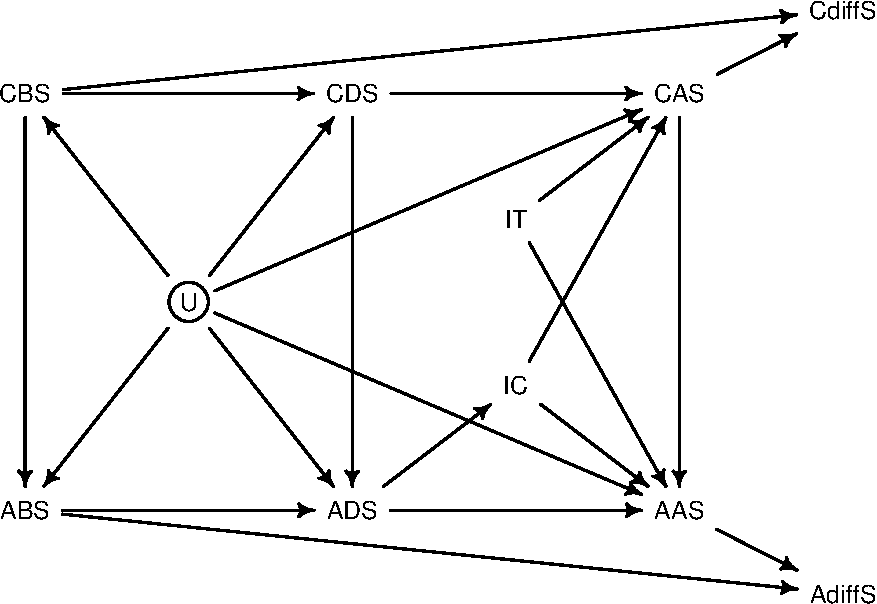
\includegraphics[width=1\linewidth]{bayesianReport_files/figure-latex/dag2-1} \end{center}

\section{Bayesian models, priors and
diagnostics}\label{bayesian-models-priors-and-diagnostics}

We will focus on a class of additive models where the outcome variable
is normally distributed around the predicted mean, which is a linear
function of predictors (possibly with some interactions). To spoil the
story, we will end up using a model, whose specification is as follows:

\begin{align*}
\mathsf{AdiffS} & \sim \textsf{Norm}(\mu, \sigma)\\
mu_i & = \alpha + \beta_{\mathsf{ADS}}[\mathsf{group}_i]\times \mathsf{ADS} + \beta_{\mathsf{group}_i}  +
 \beta_{\mathsf{IC}}[\mathsf{group}_i]\times \mathsf{IC} + \\
 & + \beta_{\mathsf{ADSIC}}\times \mathsf{ADS} \times \mathsf{IC} + \beta_{\mathsf{CBS}}[\mathsf{group}_i] \times \mathsf{CBS}\\
 \alpha & \sim \textsf{Norm}(0,.3)\\
\beta_{\mathsf{ADS}}[\mathsf{group}_i] & \sim \textsf{Norm}(0,.3)\\
\beta_{\mathsf{group}_i} & \sim \textsf{Norm}(0,.3)\\
\beta_{\mathsf{IC}}[\mathsf{group}_i] & \sim \textsf{Norm}(0,.3)\\
 \beta_{\mathsf{ADSIC}} & \sim \textsf{Norm}(0,.3)\\
 \beta_{\mathsf{CBS}}[\mathsf{group}_i]& \sim \textsf{Norm}(0,.3)\\
\end{align*}

That is, we take the resulting mean to be the result of the general
average (\(\alpha\)) and the impact of the following coefficients:
group-specific coefficient for \textsf{ADS}, group coefficient,
group-specific coefficient for \textsf{IC}, interaction coefficient for
\textsf{ADS} and \textsf{IC}, and group-specific coeffient for
\textsf{CBS}. This is plausible prima facie which group a user belongs
to might have impact on how attacks during the treatment is related to
attacks after, the role of the intervention count, and the role of
comments before. Moreover, the levels of agressive behavior displayed by
the user during treament might have impact on the role played by the
intervention count. Later on we will see that there are
information-theoretic reasons to include these interactions.

Now for the priors. One might be suspicious of \(\sigma =.3\) we
employed and suggest using standard normal distributions with
\(\sigma = 1\) instead. However, a quick prior predictive check shows
that this results in insanely wide priors that are competely
unrealistic. (For computational reasons, instead of running the
simulations, we load pre-compiled models, but we include the code used
to build them).

\vspace{1mm} \footnotesize

\begin{Shaded}
\begin{Highlighting}[]
\CommentTok{# building model with sd=1}
\CommentTok{# InteractionsModelDiffSD1 <- ulam(}
\CommentTok{#   alist(}
\CommentTok{#     AdiffS ~ dnorm( mu, sigma ),}
\CommentTok{#     mu <- a + bADS[groupID] * ADS +  bIT[groupID] + bIC[groupID] * IC+}
\CommentTok{#     bADSIC * ADS * IC+ bCBS[groupID] *CBS,}
\CommentTok{#     a ~ dnorm (0,1),}
\CommentTok{#     bADS[groupID] ~ dnorm(0,1),}
\CommentTok{#     bADSIC ~ dnorm(0,1),}
\CommentTok{#     bCBS[groupID] ~ dnorm(0,1),}
\CommentTok{#     bIT[groupID] ~ dnorm(0,1),}
\CommentTok{#     bIC[groupID] ~ dnorm(0,1),}
\CommentTok{#     sigma  ~ dexp(1)}
\CommentTok{#   ), }
\CommentTok{#   data = summaries}
\CommentTok{# )}
\CommentTok{# }
\CommentTok{# saveRDS(InteractionsModelDiffSD1, file = "models/InteractionsModelDiffSD1.rds")}
\NormalTok{InteractionsModelDiffSD1 <-}\StringTok{ }\KeywordTok{readRDS}\NormalTok{(}\DataTypeTok{file =} \StringTok{"models/InteractionsModelDiffSD1.rds"}\NormalTok{)}


\CommentTok{#now model with prior sd = .3}
\CommentTok{# InteractionsModelDiff <- ulam(}
\CommentTok{#   alist(}
\CommentTok{#     AdiffS ~ dnorm( mu, sigma ),}
\CommentTok{#     mu <- a + bADS[groupID] * ADS +  bIT[groupID] + bIC[groupID] * IC +}
\CommentTok{#     bADSIC * ADS * IC+ bCBS[groupID] *CBS,}
\CommentTok{#     a ~ dnorm (0,0.3),}
\CommentTok{#     bADS[groupID] ~ dnorm(0,.3),}
\CommentTok{#     bADSIC ~ dnorm(0,.3),}
\CommentTok{#     bCBS[groupID] ~ dnorm(0,.3),}
\CommentTok{#     bIT[groupID] ~ dnorm(0,.3),}
\CommentTok{#     bIC[groupID] ~ dnorm(0,.3),}
\CommentTok{#     sigma  ~ dexp(1)}
\CommentTok{#   ), }
\CommentTok{#   data = summaries}
\CommentTok{# )}

\CommentTok{#saveRDS(InteractionsModelDiff, file = "models/InteractionsModelDiff.rds")}

\NormalTok{InteractionsModelDiff <-}\StringTok{ }\KeywordTok{readRDS}\NormalTok{(}\DataTypeTok{file =} \StringTok{"models/InteractionsModelDiff.rds"}\NormalTok{)}

\NormalTok{##prior predictive checks sd =1}
\NormalTok{ADS <-}\StringTok{ }\DecValTok{0}
\NormalTok{CBS <-}\StringTok{ }\DecValTok{0}
\NormalTok{groupID <-}\StringTok{ }\DecValTok{1}\OperatorTok{:}\DecValTok{3}
\NormalTok{IC <-}\StringTok{ }\DecValTok{5}  \CommentTok{#mean for interventions in treatment}
\NormalTok{data <-}\StringTok{ }\KeywordTok{expand.grid}\NormalTok{(}\DataTypeTok{ADS =}\NormalTok{ ADS,}\DataTypeTok{groupID =}\NormalTok{ groupID, }\DataTypeTok{CBS =}\NormalTok{ CBS, }\DataTypeTok{IC =}\NormalTok{  IC)}
\NormalTok{prior <-}\StringTok{ }\KeywordTok{extract.prior}\NormalTok{(InteractionsModelDiffSD1, }\DataTypeTok{n =} \FloatTok{1e4}\NormalTok{)}
\NormalTok{mu <-}\StringTok{ }\KeywordTok{link}\NormalTok{( InteractionsModelDiffSD1 , }\DataTypeTok{post=}\NormalTok{prior , }\DataTypeTok{data=}\NormalTok{data ) }
\KeywordTok{colnames}\NormalTok{(mu) <-}\StringTok{ }\KeywordTok{levels}\NormalTok{(summaries}\OperatorTok{$}\NormalTok{group)}
\NormalTok{muLong <-}\StringTok{ }\KeywordTok{melt}\NormalTok{(mu)}
\KeywordTok{colnames}\NormalTok{(muLong) <-}\StringTok{ }\KeywordTok{c}\NormalTok{(}\StringTok{"id"}\NormalTok{, }\StringTok{"group"}\NormalTok{, }\StringTok{"AdiffS"}\NormalTok{)}

\NormalTok{priorGroupsSD1 <-}\StringTok{ }\KeywordTok{ggplot}\NormalTok{(muLong)}\OperatorTok{+}
\StringTok{  }\KeywordTok{geom_violin}\NormalTok{(}\KeywordTok{aes}\NormalTok{(}\DataTypeTok{x =}\NormalTok{ group, }\DataTypeTok{y =}\NormalTok{ AdiffS))}\OperatorTok{+}
\StringTok{  }\KeywordTok{theme_tufte}\NormalTok{()}\OperatorTok{+}\KeywordTok{xlab}\NormalTok{(}\StringTok{""}\NormalTok{)}\OperatorTok{+}
\StringTok{  }\KeywordTok{labs}\NormalTok{(}\DataTypeTok{title =} \StringTok{"Simulated priors by group"}\NormalTok{,}
  \DataTypeTok{subtitle =} \StringTok{"(at ADS = CBS = 0, IC at mean = 5, sd = 1)"}\NormalTok{)}\OperatorTok{+}
\StringTok{  }\KeywordTok{ylab}\NormalTok{(}\StringTok{"change in attacks (standardized)"}\NormalTok{)}

\NormalTok{ADS <-}\StringTok{ }\DecValTok{0}
\NormalTok{CBS <-}\StringTok{ }\DecValTok{0}
\NormalTok{groupID <-}\StringTok{ }\DecValTok{1}\OperatorTok{:}\DecValTok{3}
\NormalTok{IC <-}\StringTok{ }\DecValTok{0}\OperatorTok{:}\DecValTok{20}
\NormalTok{data <-}\StringTok{ }\KeywordTok{expand.grid}\NormalTok{(}\DataTypeTok{ADS =}\NormalTok{ ADS,}\DataTypeTok{groupID =}\NormalTok{ groupID, }\DataTypeTok{CBS =}\NormalTok{ CBS, }\DataTypeTok{IC =}\NormalTok{  IC)}

\NormalTok{prior <-}\StringTok{ }\KeywordTok{extract.prior}\NormalTok{(InteractionsModelDiffSD1, }\DataTypeTok{n =} \FloatTok{1e4}\NormalTok{)}
\end{Highlighting}
\end{Shaded}

\begin{verbatim}
## recompiling to avoid crashing R session
\end{verbatim}

\begin{Shaded}
\begin{Highlighting}[]
\NormalTok{mu <-}\StringTok{ }\KeywordTok{link}\NormalTok{(InteractionsModelDiffSD1 , }\DataTypeTok{post=}\NormalTok{prior , }\DataTypeTok{data=}\NormalTok{data ) }
\NormalTok{mu.mean <-}\StringTok{ }\KeywordTok{apply}\NormalTok{( mu , }\DecValTok{2}\NormalTok{, mean )}
\NormalTok{mu.HPDI <-}\StringTok{ }\KeywordTok{data.frame}\NormalTok{(}\KeywordTok{t}\NormalTok{(}\KeywordTok{apply}\NormalTok{( mu , }\DecValTok{2}\NormalTok{ , HPDI )))}
\NormalTok{priorDF <-}\StringTok{ }\KeywordTok{cbind}\NormalTok{(data, mu.mean, mu.HPDI)}
\NormalTok{priorDF}\OperatorTok{$}\NormalTok{groupID <-}\StringTok{ }\KeywordTok{as.factor}\NormalTok{(groupID)}
\KeywordTok{levels}\NormalTok{(priorDF}\OperatorTok{$}\NormalTok{groupID) <-}\StringTok{ }\KeywordTok{c}\NormalTok{(}\StringTok{"control"}\NormalTok{, }\StringTok{"empathy"}\NormalTok{, }\StringTok{"normative"}\NormalTok{)}
\KeywordTok{colnames}\NormalTok{(priorDF)[}\DecValTok{2}\NormalTok{]<-}\StringTok{ "group"}


\NormalTok{priorICSD1  <-}\StringTok{ }\KeywordTok{ggplot}\NormalTok{(priorDF, }\KeywordTok{aes}\NormalTok{(}\DataTypeTok{x =}\NormalTok{ IC, }\DataTypeTok{y  =}\NormalTok{ mu.mean,  }\DataTypeTok{fill =}\NormalTok{ group))}\OperatorTok{+}
\StringTok{  }\KeywordTok{geom_line}\NormalTok{()}\OperatorTok{+}\KeywordTok{geom_ribbon}\NormalTok{(}\KeywordTok{aes}\NormalTok{(}\DataTypeTok{ymin =}\NormalTok{ X.}\FloatTok{0.89}\NormalTok{, }\DataTypeTok{ymax =}\NormalTok{ X0.}\FloatTok{89.}\NormalTok{), }\DataTypeTok{alpha =} \FloatTok{0.2}\NormalTok{)}\OperatorTok{+}
\StringTok{  }\KeywordTok{theme_tufte}\NormalTok{()}\OperatorTok{+}\KeywordTok{ylab}\NormalTok{(}\StringTok{"change in attacks (standardized)"}\NormalTok{)}\OperatorTok{+}
\StringTok{  }\KeywordTok{labs}\NormalTok{(}\DataTypeTok{title =} \StringTok{"Simulated priors for AAS vs IC"}\NormalTok{,}
      \DataTypeTok{subtitle =} \StringTok{"(at ADS = CBS = 0, sd = 1)"}\NormalTok{)}\OperatorTok{+}\KeywordTok{xlab}\NormalTok{(}\StringTok{"interventions"}\NormalTok{)}


\NormalTok{priorJoint1 <-}\StringTok{ }\KeywordTok{ggarrange}\NormalTok{(priorGroupsSD1,priorICSD1, }\DataTypeTok{ncol =} \DecValTok{2}\NormalTok{) }
\NormalTok{priorJoint1Titled <-}\StringTok{ }\KeywordTok{annotate_figure}\NormalTok{(priorJoint1, }
  \DataTypeTok{top =} \KeywordTok{text_grob}\NormalTok{(}\StringTok{"Predictive priors with sd=1 are insanely wide"}\NormalTok{,}
                  \DataTypeTok{size =} \DecValTok{14}\NormalTok{))}
\NormalTok{priorJoint1Titled}
\end{Highlighting}
\end{Shaded}

\begin{center}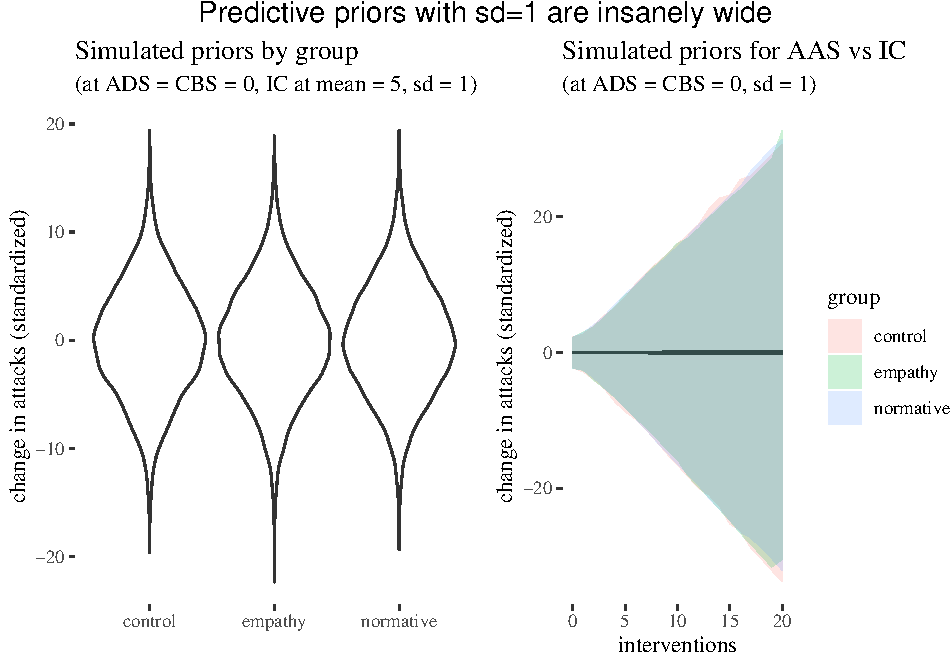
\includegraphics[width=1\linewidth]{bayesianReport_files/figure-latex/unnamed-chunk-6-1} \end{center}

\normalsize

Some experimentation leads to the value of \(\sigma =3\), which leads to
the following priors:

\vspace{1mm} \footnotesize

\begin{Shaded}
\begin{Highlighting}[]
\CommentTok{#prior predictive check sd =.3}
\NormalTok{ADS <-}\StringTok{ }\DecValTok{0}
\NormalTok{CBS <-}\StringTok{ }\DecValTok{0}
\NormalTok{groupID <-}\StringTok{ }\DecValTok{1}\OperatorTok{:}\DecValTok{3}
\NormalTok{IC <-}\StringTok{ }\DecValTok{5}  \CommentTok{#mean for interventions in treatment}
\NormalTok{data <-}\StringTok{ }\KeywordTok{expand.grid}\NormalTok{(}\DataTypeTok{ADS =}\NormalTok{ ADS,}\DataTypeTok{groupID =}\NormalTok{ groupID, }\DataTypeTok{CBS =}\NormalTok{ CBS, }\DataTypeTok{IC =}\NormalTok{  IC)}
\NormalTok{prior <-}\StringTok{ }\KeywordTok{extract.prior}\NormalTok{(InteractionsModelDiff, }\DataTypeTok{n =} \FloatTok{1e4}\NormalTok{)}
\NormalTok{mu <-}\StringTok{ }\KeywordTok{link}\NormalTok{(InteractionsModelDiff , }\DataTypeTok{post=}\NormalTok{prior , }\DataTypeTok{data=}\NormalTok{data ) }
\KeywordTok{colnames}\NormalTok{(mu) <-}\StringTok{ }\KeywordTok{levels}\NormalTok{(summaries}\OperatorTok{$}\NormalTok{group)}
\NormalTok{muLong <-}\StringTok{ }\KeywordTok{melt}\NormalTok{(mu)}
\KeywordTok{colnames}\NormalTok{(muLong) <-}\StringTok{ }\KeywordTok{c}\NormalTok{(}\StringTok{"id"}\NormalTok{, }\StringTok{"group"}\NormalTok{, }\StringTok{"AdiffS"}\NormalTok{)}
\KeywordTok{head}\NormalTok{(muLong)}

\NormalTok{priorGroupSD03 <-}\StringTok{ }\KeywordTok{ggplot}\NormalTok{(muLong)}\OperatorTok{+}
\StringTok{  }\KeywordTok{geom_violin}\NormalTok{(}\KeywordTok{aes}\NormalTok{(}\DataTypeTok{x =}\NormalTok{ group, }\DataTypeTok{y =}\NormalTok{ AdiffS))}\OperatorTok{+}\KeywordTok{theme_tufte}\NormalTok{()}\OperatorTok{+}
\StringTok{  }\KeywordTok{xlab}\NormalTok{(}\StringTok{""}\NormalTok{)}\OperatorTok{+}
\StringTok{  }\KeywordTok{labs}\NormalTok{(}\DataTypeTok{title =} \StringTok{"Simulated priors  by group"}\NormalTok{, }
  \DataTypeTok{subtitle =} \StringTok{"(at ADS = CBS = 0, IC at mean = 5, sd = .3)"}\NormalTok{)}\OperatorTok{+}
\StringTok{  }\KeywordTok{ylab}\NormalTok{(}\StringTok{"change in attacks (standarized)"}\NormalTok{)}

\NormalTok{ADS <-}\StringTok{ }\DecValTok{0}
\NormalTok{CBS <-}\StringTok{ }\DecValTok{0}
\NormalTok{groupID <-}\StringTok{ }\DecValTok{1}\OperatorTok{:}\DecValTok{3}
\NormalTok{IC <-}\StringTok{ }\DecValTok{5}  \CommentTok{#mean for interventions in treatment}
\NormalTok{data <-}\StringTok{ }\KeywordTok{expand.grid}\NormalTok{(}\DataTypeTok{ADS =}\NormalTok{ ADS,}\DataTypeTok{groupID =}\NormalTok{ groupID, }\DataTypeTok{CBS =}\NormalTok{ CBS, }\DataTypeTok{IC =}\NormalTok{  IC)}
\NormalTok{prior <-}\StringTok{ }\KeywordTok{extract.prior}\NormalTok{(InteractionsModelDiffSD1, }\DataTypeTok{n =} \FloatTok{1e4}\NormalTok{)}
\NormalTok{mu <-}\StringTok{ }\KeywordTok{link}\NormalTok{( InteractionsModelDiffSD1 , }\DataTypeTok{post=}\NormalTok{prior , }\DataTypeTok{data=}\NormalTok{data ) }
\KeywordTok{colnames}\NormalTok{(mu) <-}\StringTok{ }\KeywordTok{levels}\NormalTok{(summaries}\OperatorTok{$}\NormalTok{group)}
\NormalTok{muLong <-}\StringTok{ }\KeywordTok{melt}\NormalTok{(mu)}
\KeywordTok{colnames}\NormalTok{(muLong) <-}\StringTok{ }\KeywordTok{c}\NormalTok{(}\StringTok{"id"}\NormalTok{, }\StringTok{"group"}\NormalTok{, }\StringTok{"AdiffS"}\NormalTok{)}
\KeywordTok{head}\NormalTok{(muLong)}

\NormalTok{priorICSD03 <-}\StringTok{ }\KeywordTok{ggplot}\NormalTok{(muLong)}\OperatorTok{+}
\StringTok{  }\KeywordTok{geom_violin}\NormalTok{(}\KeywordTok{aes}\NormalTok{(}\DataTypeTok{x =}\NormalTok{ group, }\DataTypeTok{y =}\NormalTok{ AdiffS))}\OperatorTok{+}
\StringTok{  }\KeywordTok{theme_tufte}\NormalTok{()}\OperatorTok{+}\KeywordTok{xlab}\NormalTok{(}\StringTok{""}\NormalTok{)}\OperatorTok{+}
\StringTok{  }\KeywordTok{labs}\NormalTok{(}\DataTypeTok{title =} \StringTok{"Simulated priors by group"}\NormalTok{, }
  \DataTypeTok{subtitle =} \StringTok{"(at ADS = CBS = 0, IC at mean = 5, sd = 1)"}\NormalTok{)}\OperatorTok{+}
\StringTok{  }\KeywordTok{ylab}\NormalTok{(}\StringTok{"change in attacks (standardized)"}\NormalTok{)}

\NormalTok{priorJoint03 <-}\StringTok{ }\KeywordTok{ggarrange}\NormalTok{(priorGroupSD03,priorICSD03, }\DataTypeTok{ncol =} \DecValTok{2}\NormalTok{) }
\NormalTok{priorJoint03Titled <-}\StringTok{ }\KeywordTok{annotate_figure}\NormalTok{(priorJoint03, }
  \DataTypeTok{top =} \KeywordTok{text_grob}\NormalTok{(}\StringTok{"Predictive priors with sd=.3 seem sensible"}\NormalTok{,}
                  \DataTypeTok{size =} \DecValTok{14}\NormalTok{))}
\NormalTok{priorJoint03Titled}
\end{Highlighting}
\end{Shaded}

\begin{center}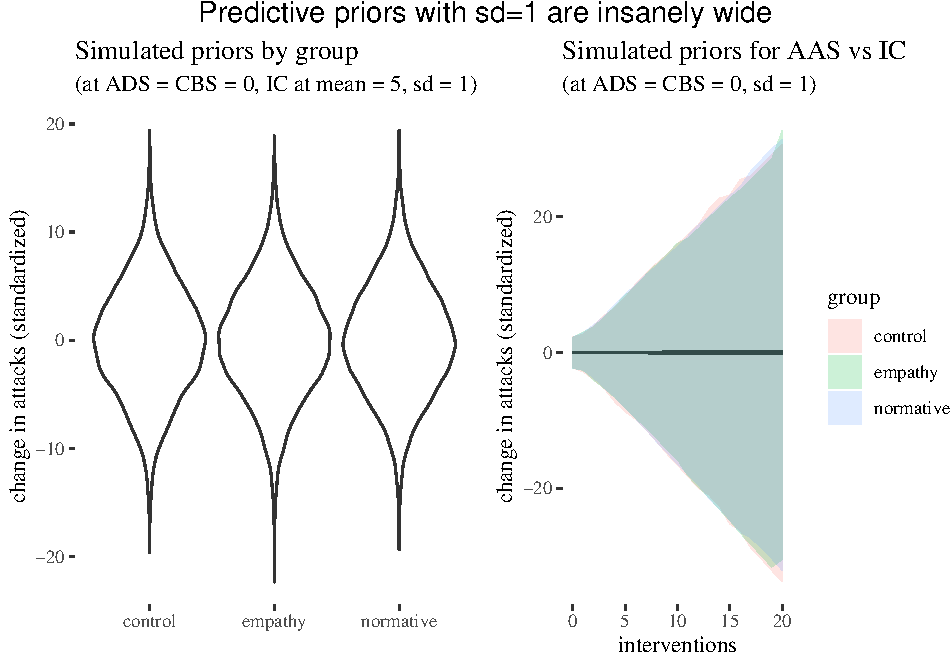
\includegraphics[width=1\linewidth]{bayesianReport_files/figure-latex/unnamed-chunk-7-1} \end{center}

\normalsize

Now, some model diagnostics before we move on. What we are witnessing is
(1) stationarity (the chains stay mostly in the most probable regions),
(2) good mixing (they explore a range of options in the beginning), and
(3) convergence (they stabilize as they progress).

\vspace{1mm} \footnotesize

\begin{Shaded}
\begin{Highlighting}[]
\KeywordTok{traceplot}\NormalTok{( InteractionsModelDiff )}
\end{Highlighting}
\end{Shaded}

\begin{center}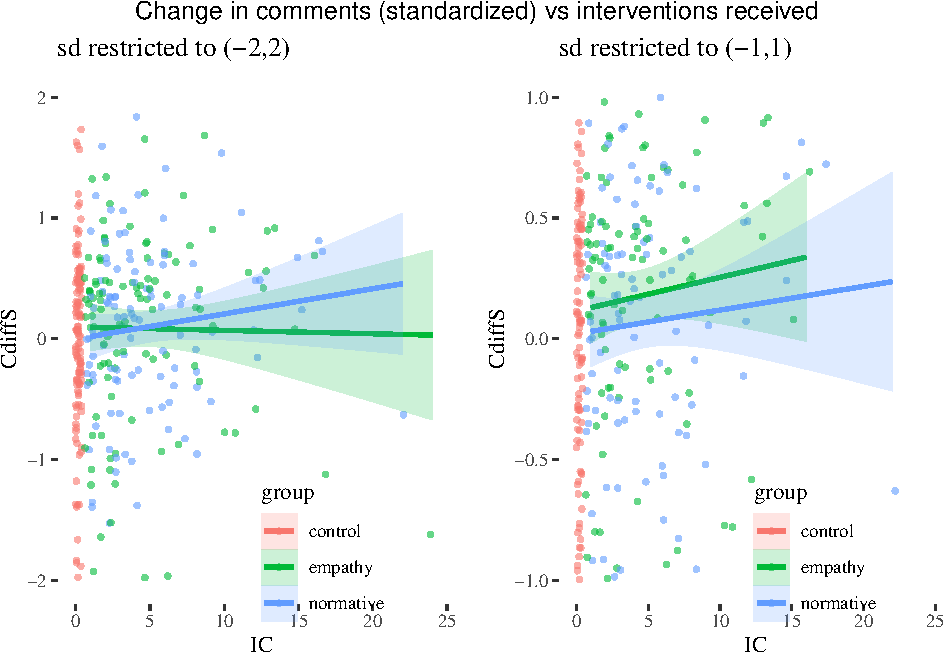
\includegraphics[width=1\linewidth]{bayesianReport_files/figure-latex/unnamed-chunk-8-1} \end{center}

\normalsize

Finally, let's inspect the distribution of residuals. That is, we
calculate all predictions, their distance from the actual values, and
inspect the distribution of the distances:

\vspace{1mm} \footnotesize

\begin{Shaded}
\begin{Highlighting}[]
\NormalTok{mu <-}\StringTok{ }\KeywordTok{link}\NormalTok{(InteractionsModelDiff)}
\NormalTok{mu_mean <-}\StringTok{ }\KeywordTok{apply}\NormalTok{( mu , }\DecValTok{2}\NormalTok{ , mean )}
\NormalTok{mu_resid <-}\StringTok{ }\NormalTok{summaries}\OperatorTok{$}\NormalTok{AdiffS }\OperatorTok{-}\StringTok{ }\NormalTok{mu_mean}
\KeywordTok{ggplot}\NormalTok{()}\OperatorTok{+}\KeywordTok{geom_density}\NormalTok{(}\KeywordTok{aes}\NormalTok{(}\DataTypeTok{x =}\NormalTok{ mu_resid))}\OperatorTok{+}\KeywordTok{theme_tufte}\NormalTok{()}\OperatorTok{+}
\StringTok{  }\KeywordTok{ggtitle}\NormalTok{(}\StringTok{"Residuals are approximately normally distributed"}\NormalTok{)}
\end{Highlighting}
\end{Shaded}

\begin{center}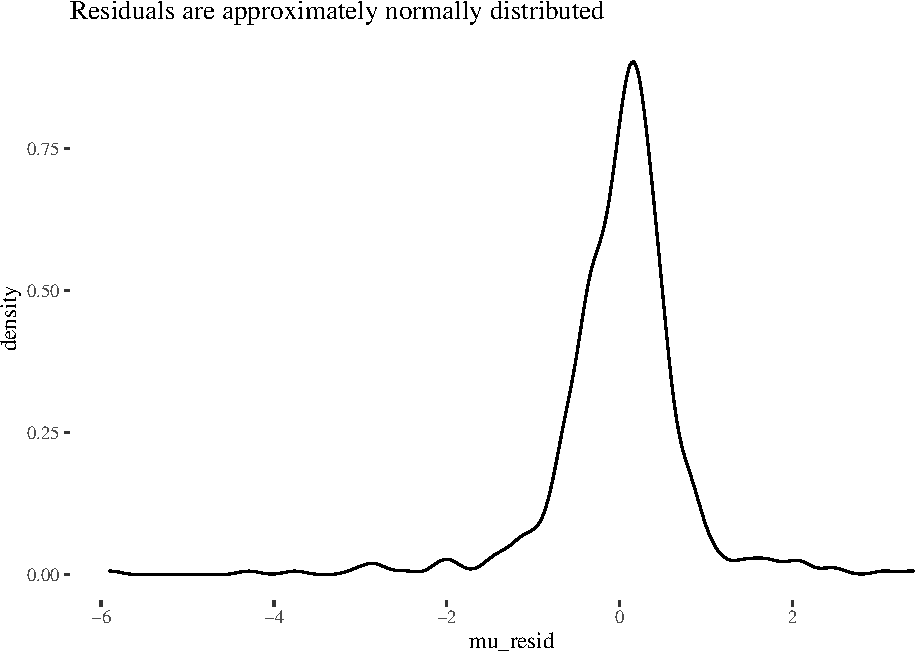
\includegraphics[width=1\linewidth]{bayesianReport_files/figure-latex/unnamed-chunk-9-1} \end{center}

\normalsize

\section*{References}\label{references}
\addcontentsline{toc}{section}{References}

\vspace{-3mm}

\end{document}
